\documentclass[main.tex]{subfiles}

\begin{document}

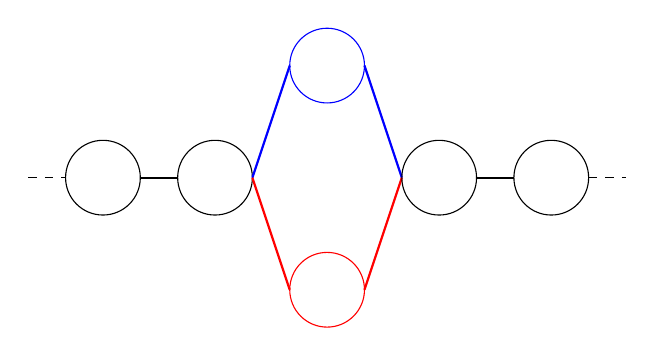
\begin{tikzpicture}[x=0.75pt,y=0.75pt,yscale=-0.9,xscale=0.9]

% begin part
\draw [dashed,black] (0, 60) -- (20, 60);
\draw (40, 60) circle (20);
\draw [fill opacity=1,thick,black] (60, 60) -- (80, 60);
\draw (100, 60) circle (20);

\draw [fill opacity=1,thick,blue] (120, 60) -- (140, 0);
\draw [fill opacity=1,thick,red] (120, 60) -- (140, 120);

\draw [blue] (160, 0) circle (20);
\draw [red] (160, 120) circle (20);

\draw [fill opacity=1,thick,blue] (180, 0) -- (200, 60);
\draw [fill opacity=1,thick,red] (180, 120) -- (200, 60);

\draw (220, 60) circle (20);
\draw [fill opacity=1,thick,black] (240, 60) -- (260, 60);
\draw (280, 60) circle (20);
\draw [dashed,black] (300, 60) -- (320, 60);

\end{tikzpicture}

\end{document}

